\documentclass[12pt]{report}
\usepackage[a4paper,top=1in, bottom=1in, left=1.5in, right=1in]{geometry} % margin
\usepackage{graphicx} %to manage figure
\usepackage{sidecap}  % for side caption of figure
\usepackage{fancyhdr} % for header and footer
\pagestyle{fancy}
\fancyhf{}
\usepackage{wrapfig} 
\rhead{ Online Training in \LaTeX} %header
\lhead{KhCE}

\begin{document}
\tableofcontents
\listoffigures
\listoftables

\chapter{Introduction}
\pagenumbering{roman}
\section{Motivation}
Start everyday with at least 5 minutes of \textbf{powerful energy}. 5 minutes of positive energy first thing in the morning can change your entire day. And if you can change your entire day with consistent positive thoughts you can change your entire life.
\textbf{\textit{Start everyday with at least 5 minutes of powerful energy. 5 minutes of positive energy first thing in the morning can change your entire day. And if you can change your entire day with consistent positive thoughts you can change your entire life.}}

\begin{figure}[h]
\centering
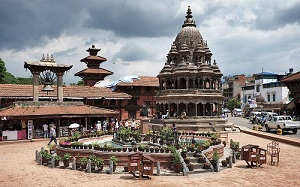
\includegraphics[scale=0.1]{patandurbar.jpg}
\caption{Patan Durbar Square}
\end{figure}

\textsc{Start everyday with at least 5 minutes of powerful energy. 5 minutes of positive energy first thing in the morning can change your entire day. And if you can change your entire day with consistent positive thoughts you can change your entire life.
Start everyday with at least 5 minutes of powerful energy. 5 minutes of positive energy first thing in the morning can change your entire day. And if you can change your entire day with consistent positive thoughts you can change your entire life.}

\underline{Start everyday with at least 5 minutes of powerful energy.}

\chapter{Placing Figure and Table}
\section{Placing Figure in \LaTeX}
Patan Durbar Square is situated at the centre of the city of Lalitpur in Nepal. It is one of the three Durbar Squares in the Kathmandu Valley, all of which are UNESCO World Heritage Sites. One of its attraction is the ancient royal palace where the Malla Kings of Lalitpur resided.

\begin{figure}[!hbt]
\centering
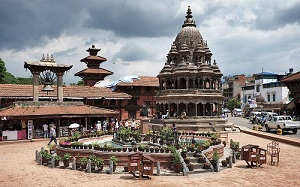
\includegraphics[scale=0.1]{patandurbar.jpg}
\caption{Patan Durbar Square}
\end{figure}

\begin{figure}[h]
\centering
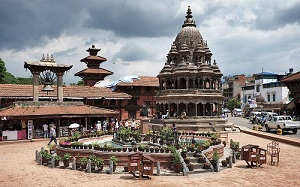
\includegraphics[width=2in,height=2in]{patandurbar.jpg}
\caption{Patan Durbar Square}
\end{figure}

Patan Durbar Square is situated at the centre of the city of Lalitpur in Nepal. It is one of the three Durbar Squares in the Kathmandu Valley, all of which are UNESCO World Heritage Sites. One of its attraction is the ancient royal palace where the Malla Kings of Lalitpur resided.
\begin{figure}[h]
\centering
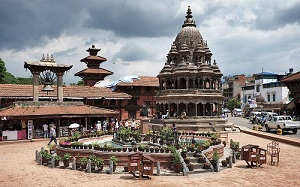
\includegraphics[scale=0.01,angle=10]{patandurbar.jpg}
\caption{Patan Durbar Square}
\end{figure}


Patan Durbar Square is situated at the centre of the city of Lalitpur in Nepal. It is one of the three Durbar Squares in the Kathmandu Valley, all of which are UNESCO World Heritage Sites. One of its attraction is the ancient royal palace where the Malla Kings of Lalitpur resided.

\begin{figure*}[!hbt]
\centering
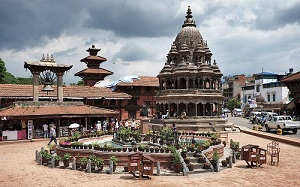
\includegraphics[scale=0.01,angle=10]{patandurbar.jpg}
\caption{Patan Durbar Square}
\label{fig:figure1}
\end{figure*}

From figure \ref{fig:figure1} Patan Durbar Square is situated at the centre of the city of Lalitpur in Nepal. It is one of the three Durbar Squares in the Kathmandu Valley, all of which are UNESCO World Heritage Sites. One of its attraction is the ancient royal palace where the Malla Kings of Lalitpur resided.

\begin{wrapfigure}{r}{0.1\textwidth} %this figure will be at the right
    \centering
    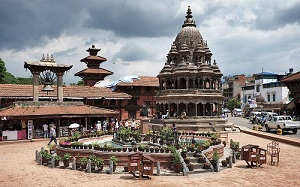
\includegraphics[width=0.1\textwidth]{patandurbar.jpg}
    \caption{Patan Durbar Square}
\end{wrapfigure}

From figure \ref{fig:figure1} Patan Durbar Square is situated at the centre of the city of Lalitpur in Nepal. It is one of the three Durbar Squares in the Kathmandu Valley, all of which are UNESCO World Heritage Sites. One of its attraction is the ancient royal palace where the Malla Kings of Lalitpur resided.
From figure \ref{fig:figure1} Patan Durbar Square is situated at the centre of the city of Lalitpur in Nepal. It is one of the three Durbar Squares in the Kathmandu Valley, all of which are UNESCO World Heritage Sites. One of its attraction is the ancient royal palace where the Malla Kings of Lalitpur resided.

\begin{wrapfigure}{l}{0.1\textwidth} %this figure will be at the right
    \centering
    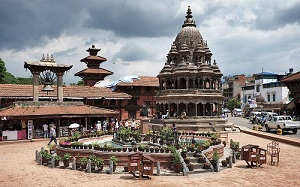
\includegraphics[width=0.1\textwidth]{patandurbar.jpg}
    \caption{Patan Durbar Square}
\end{wrapfigure}

Patan Durbar Square is situated at the centre of the city of Lalitpur in Nepal. It is one of the three Durbar Squares in the Kathmandu Valley, all of which are UNESCO World Heritage Sites. One of its attraction is the ancient royal palace where the Malla Kings of Lalitpur resided.
Patan Durbar Square is situated at the centre of the city of Lalitpur in Nepal. It is one of the three Durbar Squares in the Kathmandu Valley, all of which are UNESCO World Heritage Sites. One of its attraction is the ancient royal palace where the Malla Kings of Lalitpur resided.



\begin{figure*}[!hbt]
  
  \centering
    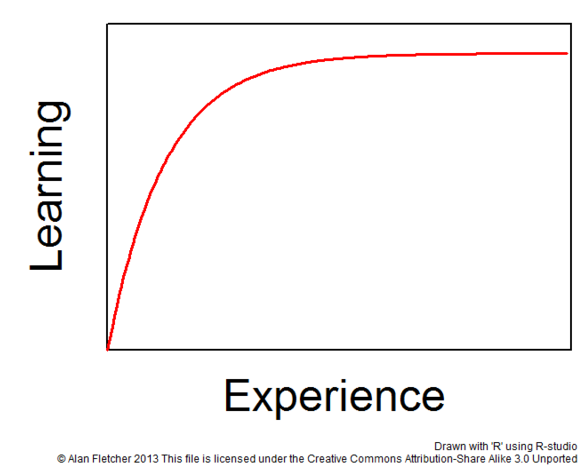
\includegraphics[width=0.5\textwidth]{figure1.png}
    \caption{IV characteristics of diode}
\end{figure*}

\begin{figure*}[!hbt]
  \centering
    \reflectbox{
      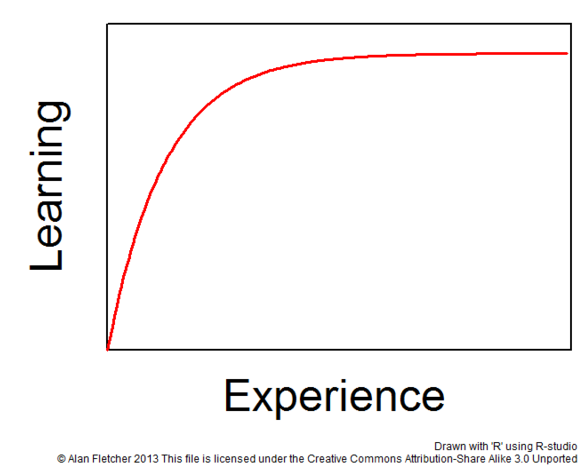
\includegraphics[width=0.5\textwidth]{figure1.png}}
  \caption{IV characteristics of diode}
\end{figure*}

\section{Placing Table in \LaTeX}

\begin{table}[!hbt]
\centering
\caption{Value of x and y}
\begin{tabular}{|c|c|}
\hline
x & y\\
\hline
1 & 2\\
\hline
3 & 4\\
\hline
5 & 6\\
\hline
\end{tabular}
\end{table}

\begin{table}[!hbt]
\centering
\caption{List of Students}

\begin{tabular}{|c|c|c|}
\hline 
S.N. & Name & Roll No \\ 
\hline 
1 & Ram  & 10 \\ 
\hline 
2 & Shyam & 40 \\ 
\hline 
3 & Hari & 50 \\ 
\hline 
4 & Sandesh & 60 \\ 
\hline 
\end{tabular} 
\end{table}

\chapter{Listing}
\section{Numbering}
\begin{enumerate}
\item Electrical Engineering
   \begin{enumerate}
   \item Power System Engineering
     \begin{enumerate}
     \item Generation
     \item Transmission
     \item Distribution
     \end{enumerate}
     
   \item Renewable Engineering
   
   \end{enumerate}

\item Computer Engineering
\item Civil Engineering
\item Electronics and Communications Engineering
\end{enumerate}


\section{Listing using bullet}
\begin{itemize}
\item Electrical Engineering
  \begin{itemize}
  \item Power System Engineering
    \begin{itemize}
    \item Generation
    \end{itemize}
  \end{itemize}

\item Computer Engineering
\item Civil Engineering
\item Electronics and Communications Engineering
\end{itemize}



\end{document}